\documentclass[main.tex]{subfiles}
\begin{document}

\usebackgroundtemplate{%
	\tikz\node[inner sep=0] {
\includegraphics[height=\paperheight,width=\paperwidth]{figures/bg}};}

\begin{frame}[c]
	\large Pengumpulan \huge Data

\end{frame}

\begin{frame}[c]
	\begin{center}
		\textcolor{red}{Statistika,}\\  \textcolor{blue}{Pengetahuan yang berhubungan dengan pengumpulan, pengolahan, penyajian dan analisa data serta pengambilan simpulan.}
	\end{center}
	\begin{textblock*}{2cm}(10cm,7cm) % {block width} (coords.12,8cm)
		
\includegraphics[width=2cm]{figures/cons}
	\end{textblock*}
\end{frame}

\begin{frame}[c]
	\frametitle{Pengumpulan Data}
	\framesubtitle{tujuan}

	\only<1>{
		\begin{description}[style=nextline]
			\item[Mengetahui jumlah elemen] Elemen :  unit terkecil dari objek penelitian, misal orang, organisasi, badan usaha, barang (unit)
			\item[Mengetahui Karakteristik]
				Karakteristik : adalah sifat , ciri atau hal yang dimiliki oleh elemen, yaitu : semua keterangan mengenai elemen.
		\end{description}}
	\only<2>{
		\textbf{Misal :}
		\begin{itemize}
			\item  elemennya pegawai swasta/pemerintah, maka karakteristiknya adalah jenis kelamin, pendidikan, agama, umur, jabatan, masa kerja dll
			\item  elemennya perusahaan, maka karakteristiknya jumlah karyawan, jumlah produksi, total penjualan 1 periode, jumlah kekayaan, dll.
			\item  elemennya universitas, maka karakteristiknya jumlah mahasiswa, jumlah dosen, banyaknya fakultas, jumlah ruang kuliah dll
		\end{itemize}
	}
\end{frame}
\begin{frame}[c]
	\frametitle{Pengumpulan Data}
	\framesubtitle{statistik}
	adalah kumpulan data dari sampel. Apabila data diambil dari keseluruhan populasi maka tidak lagi disebut statistik, melainkan parameter.

	\begin{textblock*}{2cm}(10cm,7cm) % {block width} (coords.12,8cm)
		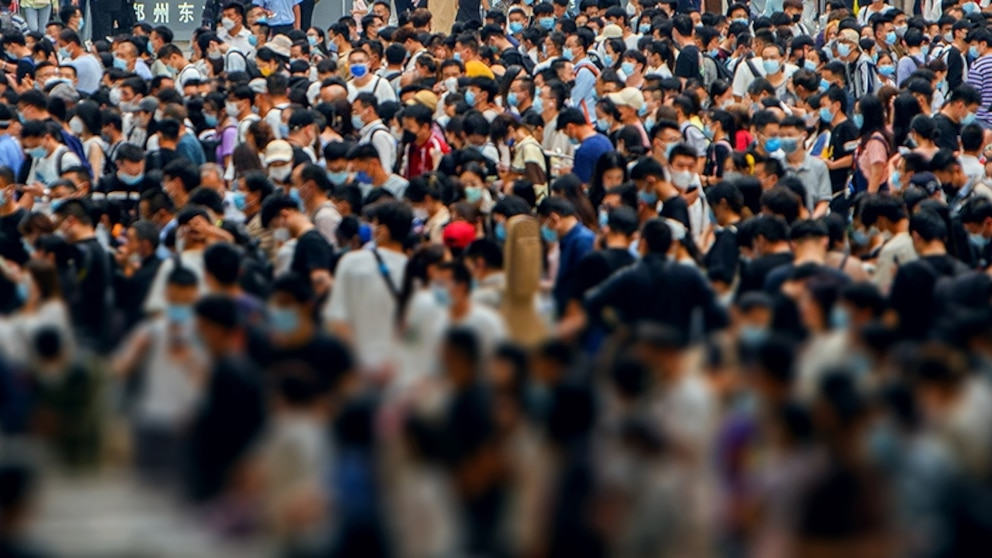
\includegraphics[width=2cm]{figures/popu}
	\end{textblock*}

\end{frame}

\begin{frame}[c]
	\frametitle{Pengumpulan Data}
	\framesubtitle{Metode}
	\begin{description}[style=nextline]
		\item[Metode Sensun]
			Metode pengumpulan data dimana seluruh elemen populasi diselidiki satu per satu.  Data yang diperoleh disebut Data sebenarnya (Parameter) atau true value. \hfill \\
			Contoh :  \textit{Sensus penduduk Indonesia tahun 1980}
		\item[Metode Sampling] Metode pengumpulan data dimana yang diselidiki adalah elemen  sampel dari suatu populasi.   Data yang diperoleh disebut  Data Perkiraan (Estimate Value).                                                        \hfill \\ Contoh :  Jika dari \textbf{1000 mahasiswa}, \textcolor{blue}{hanya 120 siswa saja yang diselidiki, maka hasilnya data perkiraan}
	\end{description}
\end{frame}

\begin{frame}[c]
	\frametitle{Populasi}
	\begin{itemize}
		\item Populasi adalah keseluruhan (totality) objek psikologi (physchological object) yang dibatasi oleh kriteria tertentu.
		\item Objek psikologis bisa merupakan objek yang bisa diraba/kongkret (tangible) maupun objek yang abstrak (untangible).
		\item Banyaknya objek psikologis dalam populasi disebut ukuran populasi (population size), yang biasanya dilambangkan dengan N
	\end{itemize}

\end{frame}

\begin{frame}[c]
	\frametitle{Sampel}
	Sampel adalah bagian dari populasi yang menjadi objek penelitian yang dianggap dapat \textcolor{pink}{mewakili  kondisi yang terjadi pada populasi.}

\end{frame}
\begin{frame}[c]
	\frametitle{Satuan Sampling}
	\begin{itemize}
		\item Sampling adalah Proses memilih objek-objek psikologis dari sebuah populasi
		\item Sampel adalah segala sesuatu yang oleh peneliti dijadikan kesatuan (unit) yang nantinya akan menjadi objek pemilihan (satuan sampling), dimana sampling bisa berbentuk individu, rumah tangga, keluarga, atau kombinasi ketiganya. Jadi sampel, adalah hasil dari proses sampling.
	\end{itemize}
\end{frame}

\begin{frame}[c]
	\frametitle{Contoh:}
	\begin{figure}
		\begin{center}
			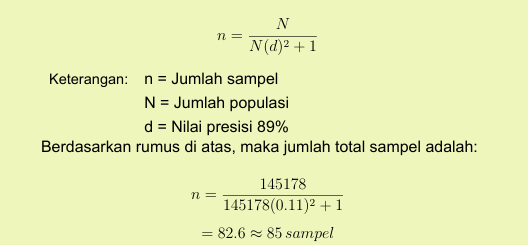
\includegraphics[height=4cm]{figures/sampelrumus}
		\end{center}
	\end{figure}
	\notec{Penelitian ini menggunakan teknik probability sampling dengan metode stratified random sampling. Metode pengambilan ini sangat cocok untuk penggalian informasi dan data dari populasi bersifat heterogen mulai dari remaja hingga orangtua. Jumlah populasi yang digunakan adalah jumlah penduduk kota Parepare pada tahun 2019, sebesar 145.178 jiwa (Bps Kota Parepare, 2020). Untuk mendapatkan jumlah sampel, maka penelitian ini menggunakan rumus Slovin dengan menetapkan nilai presesi 89\% berikut ini:}

\end{frame}

\begin{frame}[c]
	\frametitle{Ide Dasar Pengambilan Sampel}
	\begin{columns}
		\begin{column}{0.5\textwidth}
			\begin{itemize}
				\item Dengan menyeleksi bagian bagian dari elemen populasi, kesimpulan tentang keseluruhan populasi  dapat diperoleh.
				\item Sebuah eleman adalah subjek dimana pengukuran tersebut dilakukan. Ini adalah unit penelitian.
			\end{itemize}
		\end{column}
		\begin{column}{0.5\textwidth}
			\begin{itemize}
				\item Populasi adalah seluruh kumpulan elemen yang dapat digunakan untuk membuat beberapa kesimpulan.
				\item Sebuah studi sensus mencakup seluruh elemen  dalam populasi.
			\end{itemize}
		\end{column}
	\end{columns}
\end{frame}

\begin{frame}[c]
	\frametitle{Alasan Pemilihan Sampel}
	Hal-hal yang perlu diperhatikan dalam pengambilan sampel  yaitu :

	\begin{itemize}
		\item Apakah unsur populasi bersifat homogen atau heterogen.
		\item Apakah unsur populasi diketahui keberadaannya ataukah tidak.
	\end{itemize}
\end{frame}

\begin{frame}[c]
	\frametitle{Sampel yang Baik}
	Akurasi : sampai sejauh mana sampel tidak dipengaruhi bias. Jadi akurat itu artinya tidak bias.
	\begin{itemize}
		\item Sampel yang akurat adalah sampel yang dimanfaatkan untuk menyeimbangkan penilaian di antara anggota-anggota sampel.
		\item Dengan kata lain, sampel yang akurat adalah sampel yang tidak terdapat “varians sistematik”.
		\item Varians sistematik adalah variasi dalam penialian yang mengacu pada pengaruh yang diketahui, yang menyebabkan skor lebih berstandar pada satu petunjuk ketimbang yang lain.
	\end{itemize}
\end{frame}

\begin{frame}[c]
	\frametitle{Langkah Pengambilan Sampel}
	\begin{itemize}
		\item Tentukan secara jelas populasi yang menjadi sasaran penelitiannya (target population).\hfill \\
		      Populasi sasaran adalah populasi yang nantinya akan menjadi cakupan kesimpulan penelitian.
		\item Tentukan parameter penting populasi’ yaitu deskriptor (ratap-rata, varians, atau proporsi, Etc) dari variabel  dalam sebuah populasi.
	\end{itemize}
\end{frame}

\begin{frame}[c]
	\frametitle{Alat Pengumpulan Sampel}
	\begin{itemize}
		\item Daftar Pertanyaan \textit{(Questionnaire)} \hfill \\
		      \tabitem Pertanyaan tertutup \\
		      \tabitem Pertanyaan terbuka
		\item Wawancara \textit{(Interview)}
		\item Pengamatan langsung \textit{(Observation)}
	\end{itemize}
\end{frame}


\end{document}
